\documentclass{article}
\include{graphicx}
\begin{document}
%1534 words 4 and 1/2 pages

\section{Cosmological Distances}
This section introduces some of the important distances used in various prediction calculations. First of all is the comoving distance between two observers at different redshifts this is calculated via \cite{distance_measures_cosmology},
\begin{equation}
D_{C}(z)=\frac{c}{H_{0}}\int^{z_{2}}_{z_{1}}\frac{dz'}{E(z')}
\end{equation}
where E(z) is the dimensionless Hubble parameter, which general form is,
\begin{equation}
E(z)=\sqrt{\Omega_{M}(1+z)^{3}+\Omega_{R}(1+z)^{4}+\Omega_{\Lambda}}
\end{equation}
\indent Where the omegas are the different density parameters for mass, radiation and dark energy respectively.\\
\indent To calculate the comoving distance to a object at a particular redshift the integral above must be done for $z_{1}=0$ up to a arbitrary z. Comoving distance is a distance between two comoving observers i.e. both moving with respect to the Hubble flow (factoring out the expansion of the universe). In the project this has been used to determine a volume of space for a given redshift range. This was done via finding the area between two shells of radius comoving distance at two different redshifts.\\

\indent The luminosity distance is the distance a photon travels from that source. As a photon will undergo a Doppler shift and be redshifted into longer wavelengths (red part of the spectrum). Therefore the luminosity distance is essentially a redshifted transverse comoving distance (Hogg 1999), which for a flat universe is the comoving distance therefore,
\begin{equation}
D_{L}(z)=(1+z)D_{C}(z)
\end{equation}
In this project the luminosity distance has been used to convert between magnitudes, luminosity and flux.\\


\section{Schechter Function}
One important part of our project is to determine the luminosity function at high redshift, which is a plot of the number density of galaxies binned against their respective luminosity. A schechter function is used to fit this luminosity function. A schechter function is a form that has a power law which has a certain cut-off at which it becomes an exponential curve. The schechter function in terms of luminosity i.e. the luminosity function is shown below, \cite{cosmo_number_densities}.
\begin{equation}
\phi(L)=\phi^{*}\frac{L}{L^{*}}^{\alpha}e^{-L/L^{*}}
\end{equation}
\indent $\phi^{*}$ is the normalization factor in units of $Mpc^{-3}$, $\alpha$ is the gradient of the faint end slope of the luminosity function and $L^{*}$ is the characteristic luminosity at which the function changes from a power law to an exponential cut off. Therefore there are a majority of lower luminosity galaxies and not many bright ones.\\

\indent There are two basic methods to determine the best fit parameters of the schechter function \cite{luminosity_functions_online}. The first one is to take cluster samples and bin them by apparent magnitude then fit a schechter function trying to minimize the error. The other way is to use the ``maximum likelihood method''. This method takes a flux limited sample and finds the probability that a galaxy actually has a particular luminiostity at respective distances and then define a likelihood function which is the joint probability of finding all luminosities at their respective distances. These are then the most likely parameters consistent with the data and a schechter form. However in this project schechter parameters were simply cited from various articles.\\

\indent The luminosity function can then be integrated to find the number density in $Mpc^{-3}$,
\begin{equation}
\rho_{N}=\int^{\infty}_{L}\phi(L)dL
\end{equation}
Where L is the lower limit luminosity that can be seen in the universe, this is needed as the luminosity function tends to infinity at the faint end.\\
\indent It is easier to plot the luminosity function on the log scale and therefore most of the papers we cite state the absolute magnitude schechter function instead which is obtained by substituting in,
\begin{equation}
\frac{L}{L*}=10^{0.4(M^{*}-M)}
\end{equation}
which is then multiplied by the derivative and rearranged to get the equation,
\begin{equation}
\phi(M)=\phi^{*}(ln10)\left[10^{0.4(M^{*}-M)}\right]^{\alpha+1}exp\left[-10^{0.4(M^{*}-M)}\right]
\end{equation}
Where $M^{*}$ is the characteristic absolute magnitude where the cut off happens.\\
\indent However the observing team will be looking at a range of apparent magnitudes rather than absolute magnitudes and so we can change the absolute magnitude equation above to apparent using the simple relationship below,
\begin{equation}
m=M+5((log_{10}D_{L})-1)
\end{equation}
Where $D_{L}$ is the luminosity distance. Note that the derivative of this substitution is one and so does not need to be accounted for.\\

\indent Or the luminosity density of galaxies in $erg s^{-1}Mpc^{-3}Hz^{-1}$ can also be calculated using,
\begin{equation}
\rho_{L}=\int^{\infty}_{L}L\phi(L)dL
\end{equation}
This will become useful for calculating star formation rates in later sections.\\


\section{Lower Redshift limit on Reionization}
In the project the way that the lower redshift limit has been calculated is to first calculate the rate of photons capable of ionizing a hydrogen atom via the equation, \cite{2010Natur.468...49R}
\begin{equation}
\frac{dn_{ion}}{dt}=f_{esc}\zeta\rho_{SFR}  
\end{equation}
Where $f_{esc}$ is the fraction of ionizing photons that escape a galaxy, $\zeta$ is the number of hydrogen-ionizing photons produced per second per unit star formation rate and $\rho_{SFR}$ is the star formation rate per unit volume.\\
\indent Therefore by integrating this equation over the time that the universe has been around for a specific redshift a total number of photons capable of ionizing the universe can be outputted. This number is then simply equated to the number of hydrogen in the universe to get a lower redshift limit of Reionization.\\
First of all the program gets the critical density of the universe by,
\begin{equation}
\rho_{crit}(z)=\frac{3H(z)^{2}}{8\pi G}
\end{equation}
And then by multiplying this by the baryonic density parameter, $\Omega_{b}=0.045\pm0.004$, the baryonic density is achieved, which then by multiplying by the fraction of hydrogen, calculated from big bang nucleosynthesis, the total density of hydrogen in the universe can be obtained. Then finally dividing this number by the atomic mass unit to get a number density.\\

\indent In the code a redshift time relation $\frac{1}{(1+z)}\propto t^{2/3}$, assuming a matter dominated universe, is used and therefore,
\begin{equation}
t=\frac{t_{0}}{(1+z)^{3/2}}
\end{equation}
\begin{equation}
\frac{dt}{dz}=\frac{3}{2}\frac{t_{0}}{(1+z)^{5/2}}
\end{equation}

\indent In the first version of the code, values of star formation rate densities from  various articles with redshifts varying from redshifts 4 to up to about 8 from \cite{2010MNRAS.401.2561W}, which determine star formation rates from observations of Gamma-ray bursts (GRBs) from deaths of massive short lived stars which can be directly related to star formation rate. Also compiling these values with those from \cite{2012ApJ...759L..38A}, which use a semi-analytical model to determine star formation rates from redshifts 9 to 16. These two papers with very different methods have surprising correlation in values.\\
These values were then plotted against redshift. The function of redshift that was used for $\rho_{SFR}$ was,
\begin{equation}
\rho_{SFR}(z)=0.399(\pm0.181)e^{-0.253(\pm0.118)z}-0.011(\pm0.025)
\end{equation}
However this equation will only work up to a redshift of around 5 as the star formation rate for galaxies will drop with redshifts lower than this due to the ICM being used up and star formation will drop off. This should not effect our results too much however as we are looking at redshifts higher than this anyway.\\
We also used rough estimates of $f_{esc}=0.2$ and $\zeta=10^{53.5}$ obtained from \cite{2010Natur.468...49R}.\\
\indent The code then loops for different values of redshift from redshift 25 at redshift intervals of 0.1, calculating the number of ionizing photons at those different epochs and equating this to the hydrogen number. This then outputs a ionized fraction against redshift relation shown in figure \ref{fig:IonizedFraction1}.\\

\begin{figure}
	\centering
		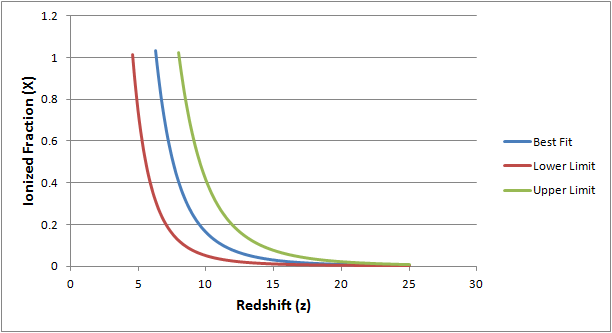
\includegraphics{F:/Extragalactic cosmology/IonizedFraction1.png}
		\caption{Plot of modeled ionized fraction of the IGM as a function of redshift.} 
	\label{fig:IonizedFraction1}
\end{figure}

From this we get that the universe is completely ionized at a redshift $7.6\pm2.1$, ignoring the rather large errors, this number is not a bad estimate of the epoch compared to articles such as from \cite{Ota:arXiv0707.1561} which shows from observations of Lyman-$\alpha$ emitters that there must be a large ionized fraction at 6.5, due to attenuation from neutral hydrogen. However this does show that this number is at a slightly higher value than what we would expect. Also as we have not included recombination which will slow down the rate at which the universe is ionized or the fact that not all the hydrogen in the universe is in the form of IGM some of it will be in the form of stars, therefore this number is not actually realistic.\\

%Next Bit to write!
\subsection{Recombinations}


@ARTICLE{2010Natur.468...49R,
   author = {{Robertson}, B.~E. and {Ellis}, R.~S. and {Dunlop}, J.~S. and 
	{McLure}, R.~J. and {Stark}, D.~P.},
    title = "{Early star-forming galaxies and the Reionization of the Universe}",
%  journal = {\nat},
archivePrefix = "arXiv",
   eprint = {1011.0727},
 primaryClass = "astro-ph.CO",
     year = 2010,
    month = nov,
   volume = 468,
    pages = {49-55},
      doi = {10.1038/nature09527},
   adsurl = {http://adsabs.harvard.edu/abs/2010Natur.468...49R},
  adsnote = {Provided by the SAO/NASA Astrophysics Data System}
}

@ARTICLE{2010MNRAS.401.2561W,
   author = {{Wyithe}, J.~S.~B. and {Hopkins}, A.~M. and {Kistler}, M.~D. and 
	{Y{\"u}ksel}, H. and {Beacom}, J.~F.},
    title = "{Determining the escape fraction of ionizing photons during Reionization with the GRB-derived star formation rate}",
 % journal = {\mnras},
archivePrefix = "arXiv",
   eprint = {0908.0193},
 primaryClass = "astro-ph.CO",
 keywords = {galaxies: high-redshift, intergalactic medium, diffuse radiation, cosmology: theory, large scale structure of Universe},
     year = 2010,
    month = feb,
   volume = 401,
    pages = {2561-2571},
      doi = {10.1111/j.1365-2966.2009.15834.x},
   adsurl = {http://adsabs.harvard.edu/abs/2010MNRAS.401.2561W},
  adsnote = {Provided by the SAO/NASA Astrophysics Data System}
}
	
@ARTICLE{2012ApJ...759L..38A,
   author = {{Alvarez}, M.~A. and {Finlator}, K. and {Trenti}, M.},
    title = "{Constraints on the Ionizing Efficiency of the First Galaxies}",
%  journal = {\apjl},
archivePrefix = "arXiv",
   eprint = {1209.1387},
 primaryClass = "astro-ph.CO",
 keywords = {cosmology: theory, dark ages, Reionization, first stars, intergalactic medium},
     year = 2012,
    month = nov,
   volume = 759,
      eid = {L38},
    pages = {L38},
      doi = {10.1088/2041-8205/759/2/L38},
   adsurl = {http://adsabs.harvard.edu/abs/2012ApJ...759L..38A},
  adsnote = {Provided by the SAO/NASA Astrophysics Data System}
}  

@article {Ota:arXiv0707.1561,
author="Kazuaki Ota and Masanori Iye and Nobunari Kashikawa and Kazuhiro Shimasaku and Masakazu A. R. Kobayashi and Tomonori Totani and Masahiro Nagashima and Tomoki Morokuma and Hisanori Furusawa and Takashi Hattori and Yuichi Matsuda and Tetsuya Hashimoto and Masami Ouchi",
title="The Reionization and Galaxy Evolution Probed by z=7 Lyman Alpha Emitters",
year="2007",
eprint="arXiv/0707.1561",
doi="10.1393/ncb/i2008-10435-8"
} 
\end{document}     